\pgfplotsset{compat=1.17}

\section{Bloom Result}
\label{sec:conc}
In the competition, we are asked to minimize the benchmarking parameter "Throughput per token including tokenize" as much as we can. To simplify the meaning of this parameter, we can describe it as : \\
\[\Phi_{token} = \frac{t_{gen} + t_{tokenize}}{n_{gen}}\]

Since the \(t_{tokenize}\) is far smaller than \(t_{gen}\), we can rewrite the equation as : \\
\[\Phi_{token} = \frac{t_{gen}}{n_{gen}}\]

In this formula, \(t_{gen}\) represents the generation time required, \(t_{tokenize}\) represents the tokenizing time required and \(n_{gen}\) is the number of new token generated. To reduce the overall throughput per token of the BLOOM inference process, we can either increase the token inlet such that more token are generated, decrease the execution time, or both.

\subsection{Batch size}
Our first strategy is increasing the total token inlet. By using Pytorch Deep Learning framework, we can easily transfer data from host to devices in pursue of better parallel ability.

Table IV lists all sentences that will be fed as the input tokens.We found that the sentences will be duplicated several times in the list until the content in the list exceeds the batch\_size. Then, we will extract the first batch\_size sentences and feed them into the language model.

\begin{table}[ht]
    \centering
    \caption{The input sentences for BLOOM inference}
    \begin{tabular}{ll}
        \toprule
        Input\_sentences  \\
        \midrule
        "DeepSpeed is a machine learning framework" \\
        "He is working on" \\
        "He got all" \\
        "Everyone is happy and I can" \\
        "The new movie that got Oscar this year" \\
        "In the far far distance from our galaxy," \\
        "Peace is the only way" \\
        \bottomrule
    \end{tabular}
    \label{table:software-GPU}
\end{table}

By experiments, we have found that the benchmarking parameter decrease as we increasing the batch\_size.

\begin{figure}
\centering
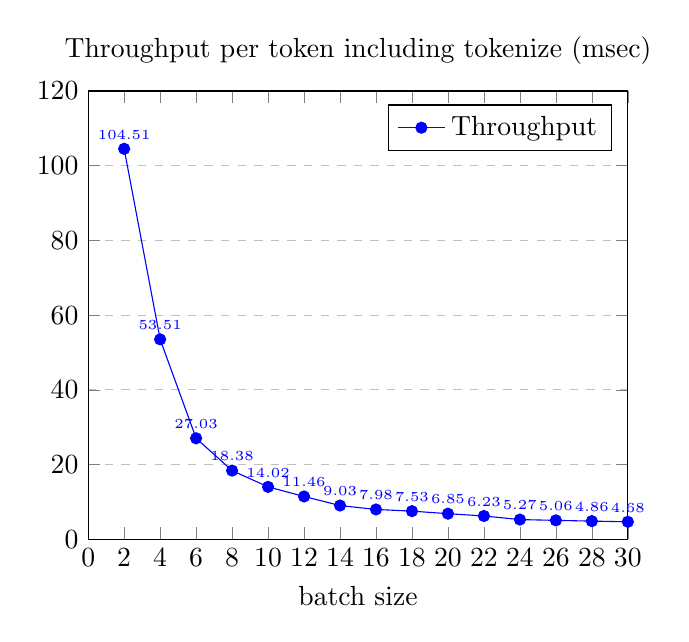
\begin{tikzpicture}
\begin{axis}[
    title={Throughput per token including tokenize (msec)},
    xlabel={batch size},
    ylabel={},
    xmin=0, xmax=30,
    ymin=0, ymax=120,
    xtick={0,2,...,30},
    ytick={0,20,40,60,80,100,120},
    legend pos=north east,
    ymajorgrids=true,
    grid style=dashed,
    every node near coord/.append style={font=\tiny},
]

\addplot[
    color=blue,
    mark=*,
    nodes near coords,
    point meta=explicit symbolic, % Allows individual points to be labeled
    ]
    coordinates {
    (2,104.51) [104.51]
    (4,53.51) [53.51]
    (6,27.03) [27.03]
    (8,18.38) [18.38]
    (10,14.02) [14.02]
    (12,11.46) [11.46]
    (14,9.03) [9.03]
    (16,7.98) [7.98]
    (18,7.53) [7.53]
    (20,6.85) [6.85]
    (22,6.23) [6.23]
    (24,5.27) [5.27]
    (26,5.06) [5.06]
    (28,4.86) [4.86]
    (30,4.68) [4.68]
    };
    \legend{Throughput}

\end{axis}
\end{tikzpicture}
\caption{Throughput per token including tokenize to batch size in two ASPIRE-2A A100x4 nodes}
\end{figure}


\subsection{Deepspeed Optimization}
Here comes another strategy. The framework we choose for Bloom is Deepspeed. It is an open-source deep learning optimization library developed by Microsoft. It is designed to enhance the training efficiency and scalability of large deep learning models. 
Deepspeed adopts three optimizations:
\subsubsection{Tensor parallelism}
In contrast, Tensor Parallelism involves the division of tensors across multiple GPUs, with each GPU handling a portion of the computation. This means that all GPUs are actively engaged in the processing simultaneously. Upon completing their respective computations, the GPUs exchange results through communication, allowing them to proceed to the next layer. By this approach, all GPUs can work simultaneously, resulting in a better overall performance.

\subsubsection{Custom CUDA Kernels}
DeepSpeed inference leverages custom CUDA kernels to minimize excessive memory allocation and inter-GPU tensor copying. As a result, this approach reduces memory requirements and decreases kernel startup overhead, leading to improved throughput and the ability to work with larger batch sizes, ultimately resulting in higher overall throughput.

\subsubsection{Mixture of Quantization}
Mixture of Quantization involves loading INT8 data from memory and converting it to FP16 before utilizing it in inference computations. This approach leverages the BitsAndBytes Python package to achieve these conversions. The key advantages include model size reduction and a substantial decrease in the inference cost during production.

\subsection{NCCL Optimization}
Here are some NCCL environment variables that we have found useful.
\subsubsection{NCCL\_NET\_GDR\_READ}
We set this variable to 1 (default 0 in non-NVlink based platform) to use GPU Direct RDMA to send data to the NIC directly.
\subsubsection{NCCL\_IB\_QPR\_PER\_CONNECTION}
We set this variable to "SYS" to always enable GPU Direct RDMA even across NUMA nodes.
\subsubsection{NCCL\_NTHREADS}
By default, V100 on Gadi use 256 threads only. We set this variable to 512 to enlarge the CUDA threads per CUDA blocks. Increasing this variable can increase the GPU clock rate.
\subsubsection{NCCL\_BUFFSIZE}
This variable control the size of buffer used by NCCL when communicating between pairs of GPUs. By experiment, we have found that setting buffer size to 8Mb gives the best performance on Gadi.



\subsection{Comparison between Gadi and Taiwania2}

\begin{figure}[h!]
\centering
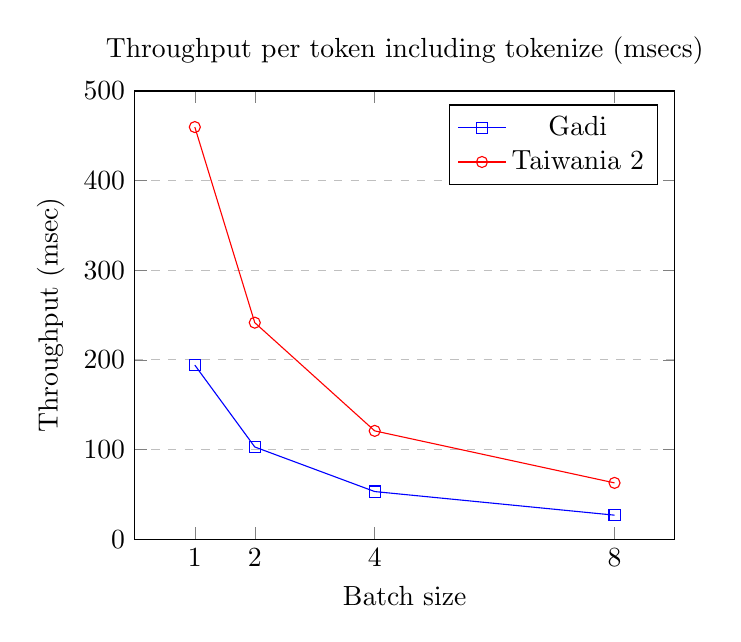
\begin{tikzpicture}
\begin{axis}[
    title={Throughput per token including tokenize (msecs)},
    xlabel={Batch size},
    ylabel={Throughput (msec)},
    xmin=0, xmax=9,
    ymin=0, ymax=500,
    xtick={1,2,4,8},
    ytick={0,100,200,300,400,500},
    legend pos=north east,
    ymajorgrids=true,
    grid style=dashed,
]

% Gadi data
\addplot[
    color=blue,
    mark=square,
    ]
    coordinates {
    (1,194.23)(2,102.93)(4,53.2)(8,26.87)
    };
    \addlegendentry{Gadi}

% Taiwania 2 data
\addplot[
    color=red,
    mark=o,
    ]
    coordinates {
    (1,459.72)(2,241.56)(4,120.88)(8,62.87)
    };
    \addlegendentry{Taiwania 2}

\end{axis}
\end{tikzpicture}
\caption{Comparison of throughput for Gadi and Taiwania 2 across different batch sizes.}
\end{figure}


\subsection{Unsuccessful Attempts}
We've also tried to use some optimization tools provided by NVIDIA, but failed to achieve any significant improvement in our results.
\subsubsection{FasterTransformer}
We've tried FasterTransformer since it claims that it provides some optimizations such as layer fusion, caching, support of multi-node, matmul kernel auto-tunning, etc.
However, it didn't have directly support of our BLOOM-176B model. Therefore we turned to other tools after successfully building the required image.
\subsubsection{TensorRT}
We've also tried TensorRT, which we thought can make use of the TensortRT inference engine to improve the performance.
It first requires to convert BLOOM to ONNX format. Unfortunately, BLOOM-176B is such a large model that it's lots of work for us to transform the entire model. We make a pause after converting the first layer of BLOOM-176B.
\subsubsection{TensorRTLLM}
Our last attempt was TensorRTLLM, which was just released recently. We thought it was the most suitable tool for us to use as its name showed. Not only it incorporates the desirable optimizations, such as kernel fusion, Tensor engine, ... some formally provided by FasterTransformer and TensorRT, it also provides python API and direct support of BLOOM-176B.
Thought finding such powerful tool, we still fail to build TensorRT engine due to memory issue, as we encountered when using TensorRT.

To sum up, almost all the attempts failed due to insufficient memory, which is unsolvable. Therefore, although they provide many desirable optimizations, these tools are not feasible in our cases.